\documentclass[11pt]{report}
\usepackage[utf8]{inputenc}
\usepackage{csquotes} % Add this line to import the 'csquotes' package
\setcounter{tocdepth}{3}
\setcounter{secnumdepth}{3}
\usepackage{graphicx} % Required for inserting images
\usepackage{appendix}
\usepackage{sectsty}
\usepackage{paperStyle}
\usepackage{tabularx}
\usepackage{siunitx}
\usepackage{tipa}
\usepackage{textcmds}
\usepackage{multirow}
\usepackage{float}
\usepackage[dvipsnames]{xcolor}
\usepackage{soul}
\definecolor{HLColor}{RGB}{230,230,250}
\sethlcolor{HLColor}
\usepackage[
    backend=biber,
    style=numeric,
    sorting=none
  ]{biblatex}

% TOP MARGIN:
\makeatletter
\setlength{\@fptop}{0pt}
\makeatother

% BIBLIOGRAPHY:
\addbibresource{references.bib}

% TITLE:
\title{\Huge \textbf{Mood Tracker}\vspace{2mm} \\
    \large Part 1: User Interface Design}

% AUTHORS:
\author{\vspace*{1cm}\Large Alexandros Tsaparas
\\ \textit{Supervisor: Christos Sintoris}
\and Electrical and Computer Engineering Department,
\\University of Patras\vspace{5mm} \\
AM: 1072824}
\date{}

\begin{document}
\maketitle 
\tableofcontents

\chapterfont{\LARGE \centering}
\chaptertitlefont{\Large \centering}
\chapter{User research - Key problems}

\section{Introduction to the Mood Tracker app}

In the following, the basic principle of the app is presented in order to be able to better classify all procedures and results of the user research and problem identification in the topic field.\\
The core premise of the application revolves around the identification of issues and concerns through regular anonymous surveys administered to university students. Furthermore, it aims to provide initial ideas and thoughts to improve the overall student environment. My Moodtracker app is specifically designed for universities interested in students satisfaction. Survey results are provided to professors in a completely anonymous format. Students can view their survey history and analyze how their answers have changed over time. In addition, there should still be a way for students to contact their supervisors directly to communicate individual ideas and suggestions.\\
Finally, it's worth mentioning that although a majority of the features will be incorporated and additional ones may be introduced throughout the complete app development process, it's possible that not all of them will be included in the final prototype.

\section{Preparatory Research}

The following item deals with the relevance of our app as well as the user research. In particular, it discusses why student satisfaction is important for universities. For this purpose, various scientific articles and publications as well as contributions from health-related organizations were considered. In addition, an exemplary survey was conducted in order to be able to specifically address user requirements when designing the app.

\subsection{Relevance of a Moodtracker for Universities}

In the course of my user research, I found numerous sources that prove that student well-being is directly related to their productivity. For this reason, student satisfaction and mental health is an increasingly important factor for universities.\\
Many qualitative studies have been conducted at different universities.

\subsubsection{First research}

\textbf{University of Applied Sciences, Northern Netherlands \cite{research-1}}
\\ \normalsize Taking advantage of the high number of students who study at their institution, they collected data through in-depth and open-ended interviews between May and November 2020 (beginning of the COVID-19 pandemic).\vspace{5mm} \\
\textbf{Method} \\
The institution made sure to inform the students through researchers (intranet messages) and Heads of School. A total of 113 students signed up for interviews, selected through purposive sampling based on criteria like full-time status, well-being problems, and diverse representation. Participants were from various academies, study years, and genders. Interviews, lasting 28 to 52 minutes, explored student well-being and related factors. Consent was obtained, and interviews were video recorded. The semi-structured guide covered topics such as defining well-being and factors influencing it. Data collection continued until saturation, with 27 students interviewed.\vspace{5mm} \\
\textbf{Analysis} \\
Thematic analysis was used to interpret data, involving verbatim transcription, member checks, and independent coding by three researchers. Coding was initially done line by line using an open coding approach, with the possibility of applying multiple codes to a passage. Codes were then organized into categories based on data and literature concepts, forming themes. Categories, themes, and data allocation were verified in the final phase by two other researchers to ensure clarity and consistency. Discussions resolved any discrepancies until an agreement was reached.\vspace{5mm} \\
\textbf{Results} \\
Participated five male students, twenty-one female students, and one non-binary student, all aged between 17–24 years, participated. There was revealed a diverse range of self-reported well-being issues among the participating students. These included challenges such as inadequate support from the school, anxiety disorders, family-related issues, physical health problems, symptoms of depression, gender dysphoria, fatigue, and performance anxiety. Additionally, factors like stress, planning difficulties, study pressure, loneliness, perfectionism, and getting used to studying were frequently mentioned by the students. Some participants highlighted the impact of life phase-related problems, ADHD, and drug use on their well-being. The findings underscore the complexity and multifaceted nature of the well-being issues faced by students, emphasizing the need for a holistic approach in addressing these concerns, both within and beyond the academic environment.\vspace{5mm} \\
\textbf{Students' opinions} \\
They expressed diverse views on student well-being. Initially, some found it challenging to define, but as interviews progressed, themes emerged. Well-being was associated with managing stress, achieving balance in academic and personal life, and acknowledging the effort-achievement ratio. Stress and resilience were central themes, with students emphasizing the need to cope with challenges. Well-being was seen as a combination of mental, physical, and social aspects, with support from the university playing a crucial role. Students acknowledged the fluctuating nature of well-being and its significant impact on academic performance.\vspace{5mm} \\
\textbf{Main Factors} \\
The main factors influencing student well-being include self-regulation, perfectionism, motivation levels, ability to plan, and study achievements at the individual level. Fellow students contribute to well-being through practical support, idea exchange, enjoyment, and fostering a community atmosphere. Tutors play a crucial role with good relationships, trustworthiness, accessibility, and time availability. Attitudes and behaviors such as empathy, guidance, and personal attention also influence well-being. Teachers impact well-being through good relationships, accessibility, informal contact, community atmosphere, and attitudes like reassurance, understanding, and recognition. Study-related factors include clear communication, flexibility, workload, and the scale of education. The university's support facilities and community atmosphere are significant. Peers outside the university contribute to well-being through enjoyment, idea exchange, understanding, and recognition. Family support, idea exchange, and enjoyment are also key factors.

\subsubsection{Second research}

\textbf{Renmin University of China, Haidian, Beijing, China \cite{research-2}}
\\ \normalsize The university conducted research on students' well-being, recognizing the importance of mental health in maintaining overall health. The study addresses the global rise in depression and anxiety cases, particularly among college students. College is identified as a critical period for shaping values, and students' emotional well-being is linked to various factors. The research aims to understand changing trends in students' negative emotions over four academic years by analyzing a cohort from 15 Chinese universities. This study seeks to offer valuable insights for providing appropriate guidance and support to enhance students' well-being during their college  years.\vspace{5mm} \\
\textbf{Method} \\
This study employed data from the "Beijing College Student Panel Survey" within the "China Education Panel Survey," focusing on the 2008 cohort of students tracked for four years from 2009 to 2012. Sampling involved 15 universities, and the effective sample size was 1401 students. The investigation utilized the Depression Anxiety Stress Scales-21 (DASS-21) to assess psychological well-being, a self-report measure known for its reliability. The DASS-21 includes three scales for depression, anxiety, and stress, each comprising seven items. Scores are calculated by summing corresponding item scores. Notably, the DASS-21's short version requires scores to be multiplied by two for comparison with conventional severity ratings. The study reported good validity for the DASS measurement, supported by scale reliability coefficients of 0.813 for depression, 0.766 for anxiety, and 0.812 for stress. Overall, the methodology involved a comprehensive survey approach, online and on-site rounds, and rigorous measures for assessing students' mental health across their college years.\vspace{5mm} \\
\textbf{Results} \\
The results from the study, provide insights into the mental well-being of Chinese college students across four academic years. The average scores for depression and stress, ranging between 7.22 and 7.79 for depression and 9.53 and 11.68 for stress, consistently fell within the normal range based on cutoff values. However, anxiety scores in the first three years slightly surpassed the normal threshold of 7, with mean scores of 7.40, 7.24, and 7.10, indicating above-average anxiety levels. The previously mentioned statistic numbers, as they increase they reflect more and more the severity of depressive and stress-related symptoms. Interestingly, anxiety levels seemed to decrease in the senior year, with a mean score of 6.63. Despite above-normal anxiety levels in the initial years, students maintained mental health with depression and stress scores in the normal range. The study suggests a fluctuation in mental states, with students experiencing higher stress and depression in the sophomore year, while improvements were observed in the last two years. These findings shed light on the dynamic nature of college students' mental well-being over their academic journey, emphasizing the need for targeted interventions and support to enhance mental health throughout their college experience.\vspace{5mm} \\
\textbf{Discussion and Conclusion} \\
In conclusion, the study sheds light on the mental well-being of Chinese college students over four academic years. Freshmen and sophomores exhibited more mental health challenges, possibly stemming from adjustment issues and increased study pressures. Financial concerns were identified as a significant contributor to anxiety, with Chinese students having relatively lower financial burdens compared to their UK counterparts. Notably, the study revealed differences in psychological well-being trends between China and the US, emphasizing the need for tailored interventions. The longitudinal approach strengthened the credibility of the findings, highlighting grade-related disparities. Key conclusions include the average mental health of Chinese college students, their vulnerability to anxiety in the initial years, and the improvement in psychological well-being over time. The study recommends targeted psychological guidance for different academic years, emphasizing the importance of addressing anxiety in freshmen and enhancing well-being support for sophomores. Future research may explore students' mental changes after entering the workforce for further insights into the development of psychological well-being counseling programs in college.

\subsubsection{Concluding Insights on Student Well-Being in Higher Education}

In distilling insights from diverse university research studies on student well-being, a stark reality surfaces, unveiling the intricate challenges that students in higher education confront. The imperative of adopting a student perspective, as underscored by Douwes et al. \cite{research-1} and Liu et al. \cite{research-2}, emphasizes the urgency of comprehending well-being from the direct vantage point of those immersed in university life. Both investigations expose a disconcerting trend: students' psychological well-being undergoes discernible fluctuations amid the labyrinth of academic expectations, workload pressures, and examination stressors. Furthermore, the incorporation of established scales, such as the Short Warwick-Edinburgh Mental Well-Being Scale and the Perception of Academic Stress Scale, provides an unflinching framework, casting light on the prevailing issues of mental health and academic stress.
\\"The student well-being model" proposed by Soutter et al. \cite{research-3} contributes significantly to the arsenal of tools for gauging student well-being. Drawing from empirical and theoretical research, the authors present a nuanced model considering diverse domains and categories that impact students' well-being. This framework stands as an indispensable instrument for educators, researchers, and policymakers, urging them to recognize and elevate student well-being in educational settings. Conversely, Hascher's \cite{research-4} research on quantitative and qualitative approaches to assess student well-being spotlights a concerning reality: a lack of a specific definition and assessment of well-being in the school context. The study introduces innovative tools, including a multi-faceted well-being questionnaire and emotion diaries, offering a holistic evaluation of well-being in school.
\\These studies collectively underscore the pressing need to confront the unsettling status quo of students' well-being in higher education. The synthesis of empirical evidence and theoretical frameworks lays bare the interconnected nature of factors influencing well-being, spanning academic, emotional, and social dimensions. Strikingly, the research paints a picture where universities and educators appear oblivious or inert to the burgeoning well-being crisis. As educational institutions strive to foster supportive learning environments, the revelations from these studies should serve as a clarion call for substantive interventions and policies aimed at ameliorating the comprehensive well-being of students in higher education.


\subsection{Survey as a Tool for User Research}

My survey should help me identify the problems my application can solve and figure out how I can optimize its design to achieve the best result. I chose to design the survey with both quantitative and qualitative questions, such as rating scales and open-ended inquiries, in order to have a better understanding of the participants' experiences. It also has comprehensive range of questions addressing various aspects of the academic experience, making it well-rounded and insightful.

\begin{figure}[h!]
    \centering
    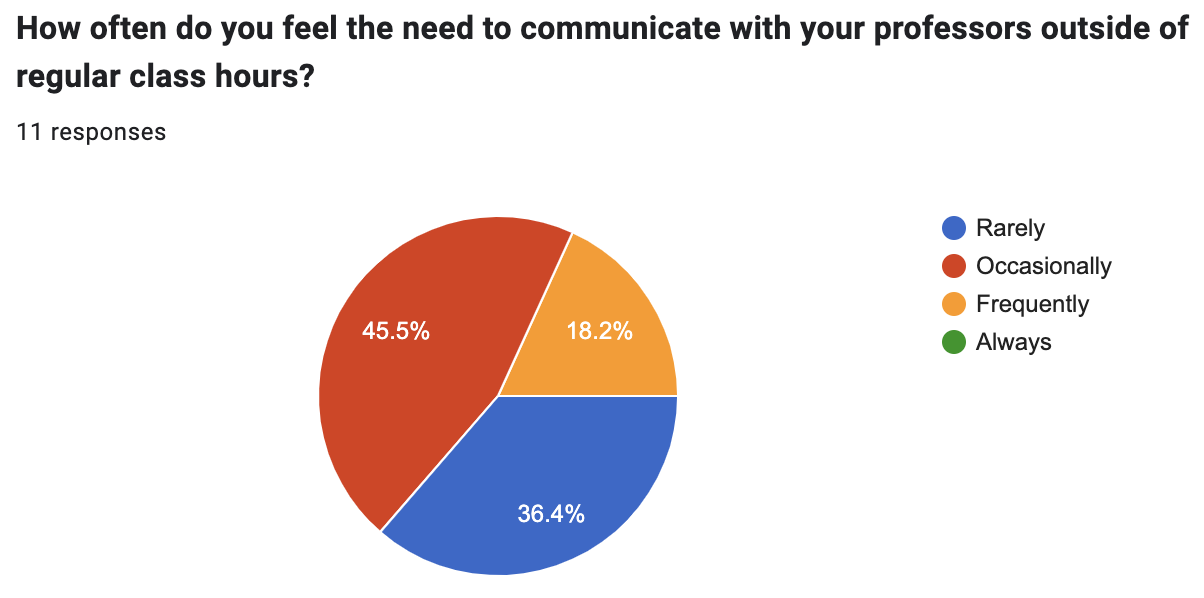
\includegraphics[width=0.9\linewidth]{figures/results/q11.png}
    \caption{Enter Caption}
    \label{fig:comments form}
\end{figure}

\subsubsection{Realization of the Survey}

\subsubsection{Results of the Survey}

\section{Comparative Analysis of Existing Mood-Tracking Apps}

In my exploration of the most used mood-tracking apps of 2023, I encountered several noteworthy options with distinct strengths and weaknesses. \textbf{\href{https://www.getmoodfit.com/}{Moodfit}}, while lacking in consistency in interface appeal, presents valuable features such as charts and meditation exercises that could enrich the user experience in my app. \textbf{\href{https://worrywatch.com/}{Worry Watch}}, though limited to iOS and featuring a challenging interface, offers positive affirmations—an aspect that could inspire a focus on mental well-being in my application. Also offers exercises (breathing, meditation) with a variety of options/modifications that create a safe place for the user. \textbf{\href{https://www.moodtools.org/}{MoodTools}}, while maintaining a simple design, could benefit from a more refined frontend and interactive elements, which my app aims to incorporate for enhanced engagement. \textbf{\href{https://mobile.va.gov/app/ptsd-coach}{PTSD Coach}}, tailored for military service members, showcases an appealing interface and color palette, influencing my consideration for a visually pleasing design. \textbf{\href{https://emoodtracker.com/}{eMoods (Bipolar Mood Tracker)}}'s complex interface and subscription-based full version might prompt my app to emphasize user-friendly design and affordability. Also is a more specialized app, specific to bipolar disorder (hence the name). \textbf{\href{https://www.thriveport.com/products/moodkit/}{MoodKit}}, despite its outdated interface, provides password-protected journals and charts, influencing my app's focus on security and comprehensive mood tracking. \textbf{\href{https://daylio.net/}{Daylio}}'s simplicity and color scheme align with my app's objectives, while its inclusion of emoji answers could inspire a similar interactive approach.

\section{Conclusion}

Building upon the insights gathered from the aforementioned articles on students' moods in universities and our comprehensive survey aimed at uncovering the most pressing issues affecting their well-being, our mood-tracking application takes a pioneering approach. The information gleaned from these sources has been instrumental in shaping a solution that not only combines the best features from existing apps but also digs into the core challenges faced by students in the university environment.\vspace{5mm} \\
The combination of these sources has enabled our application to transcend the limitations observed in current solutions. It aims to provide an unparalleled, user-friendly experience that not only visually captivates users but also serves as a powerful tool for understanding and anonymously tracking students' moods efficiently. Our solution is not merely an integration of features; it is a thoughtful response to the intricate interplay of factors influencing the emotional landscape of students in higher education.

\section{Appendix - The survey as presented to the participants}

The survey's first page [\ref{fig:q1}] introduces the research purpose, expresses gratitude to participants, and underscores the importance of their insights in understanding academic challenges. Clear instructions urge participants to share thoughts confidentially, emphasizing the positive impact on creating a more supportive university experience.\vspace{5mm} \\
The second page [\ref{fig:q2}] is all about collecting basic personal information that aims to discern whether university challenges have a uniform impact on the mood of all students or if specific groups are more susceptible.\vspace{5mm} \\
The third page [\ref{fig:q3}] of the survey digs into the academic experiences of participants, by asking a comprehensive set of questions aims to capture nuanced aspects of the academic experience and stressors that contribute to a holistic understanding of the challenges students may face.
\begin{figure}[h!]
    \centering
    \subfloat[First]{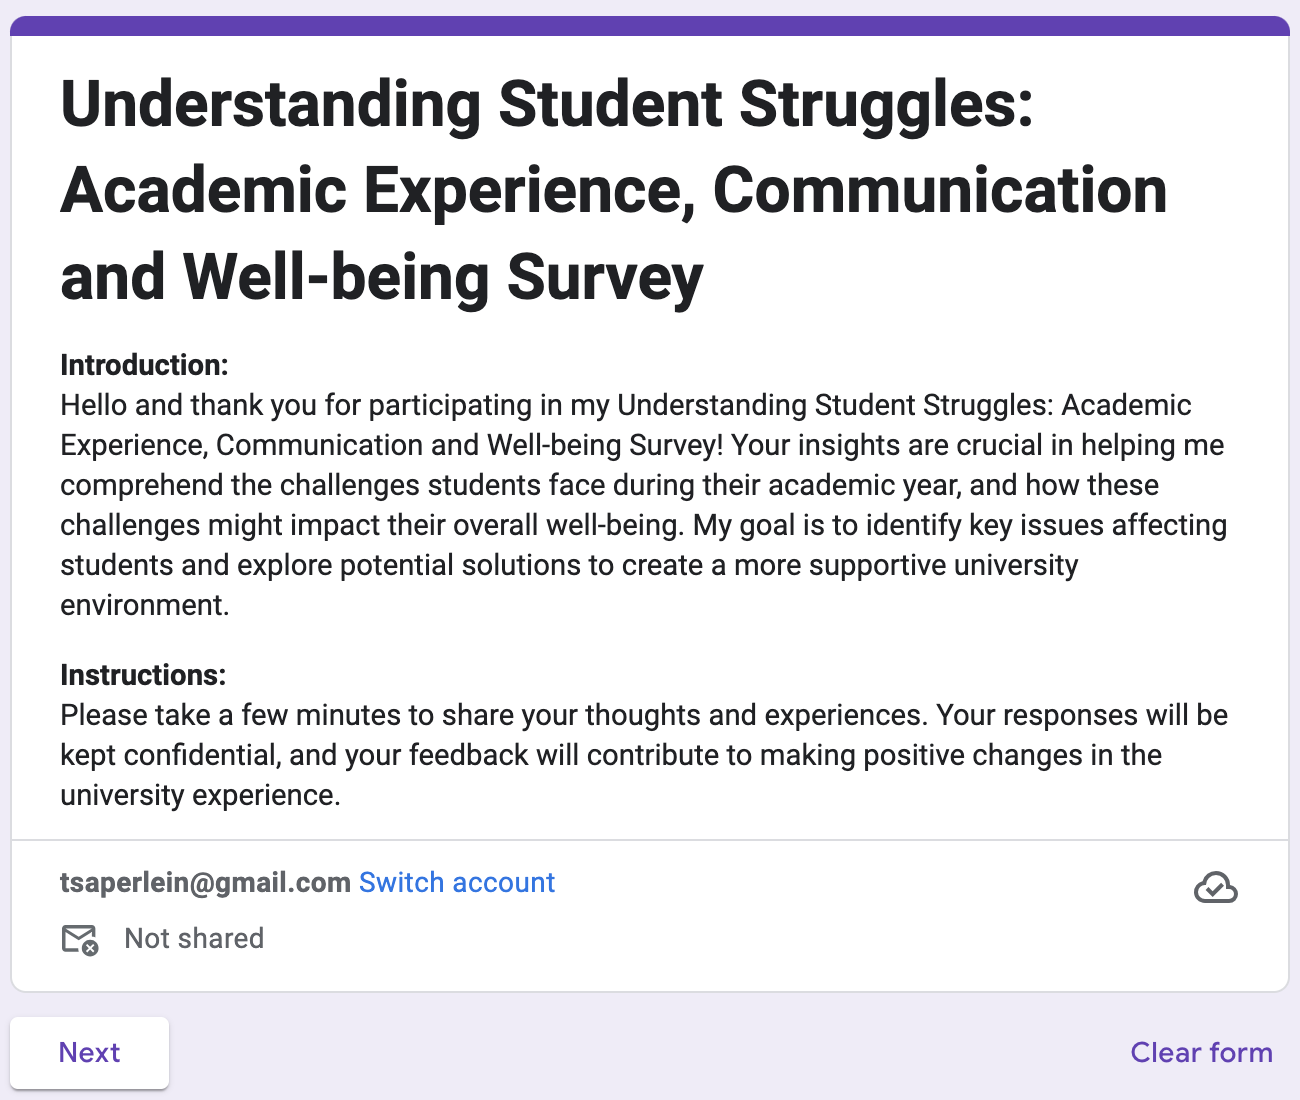
\includegraphics[width=0.52\linewidth]{figures/images/1.png}\label{fig:q1}}
    \hfill
    \subfloat[Second]{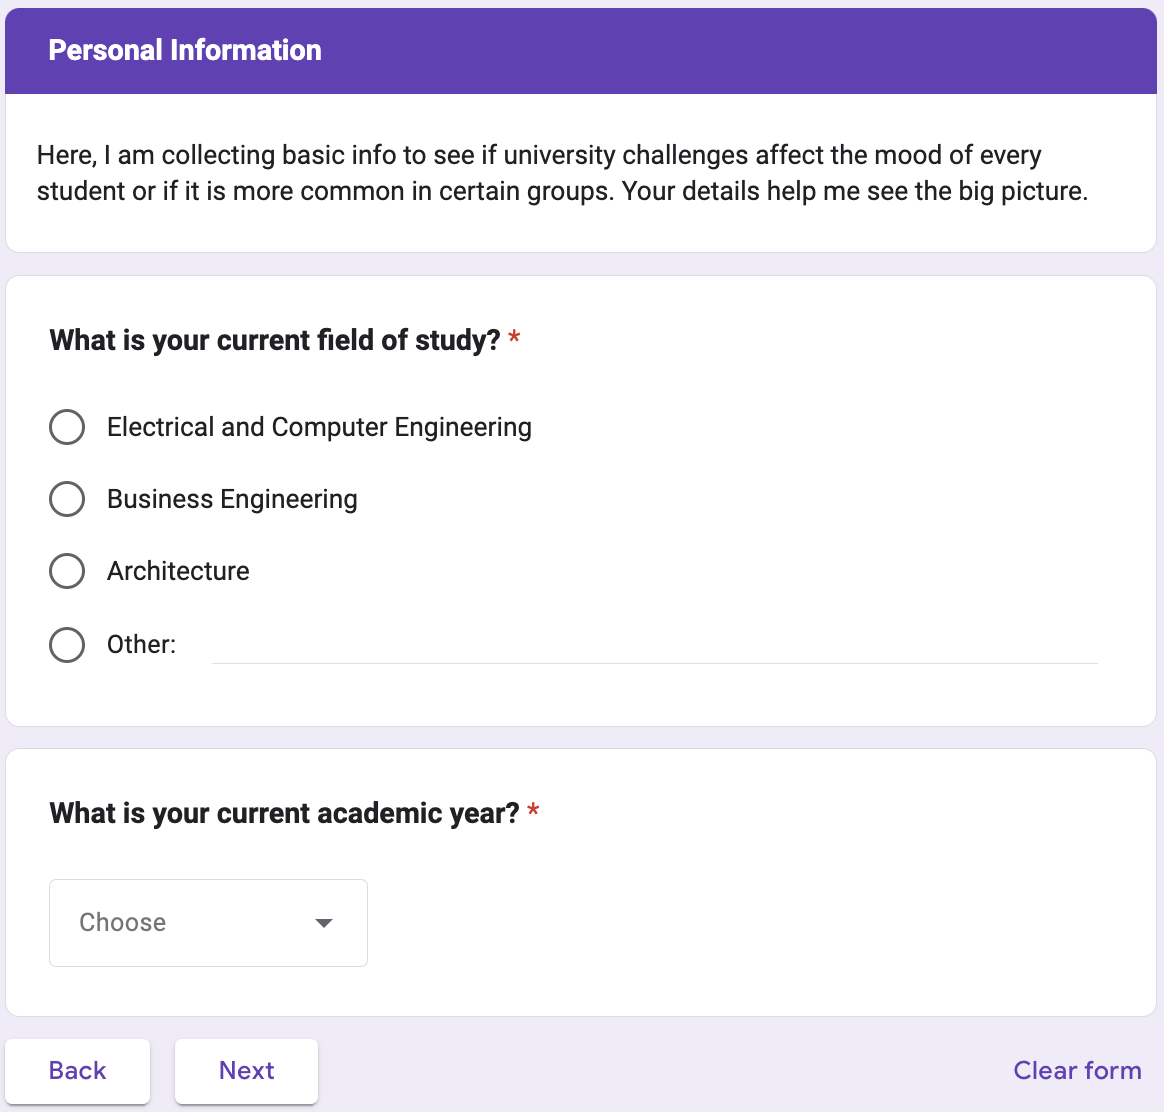
\includegraphics[width=0.46\linewidth]{figures/images/2.png}\label{fig:q2}}
    \caption{First and second page of the survey}
\end{figure}
\begin{figure}[h!]
    \centering
    \subfloat[Part 1]{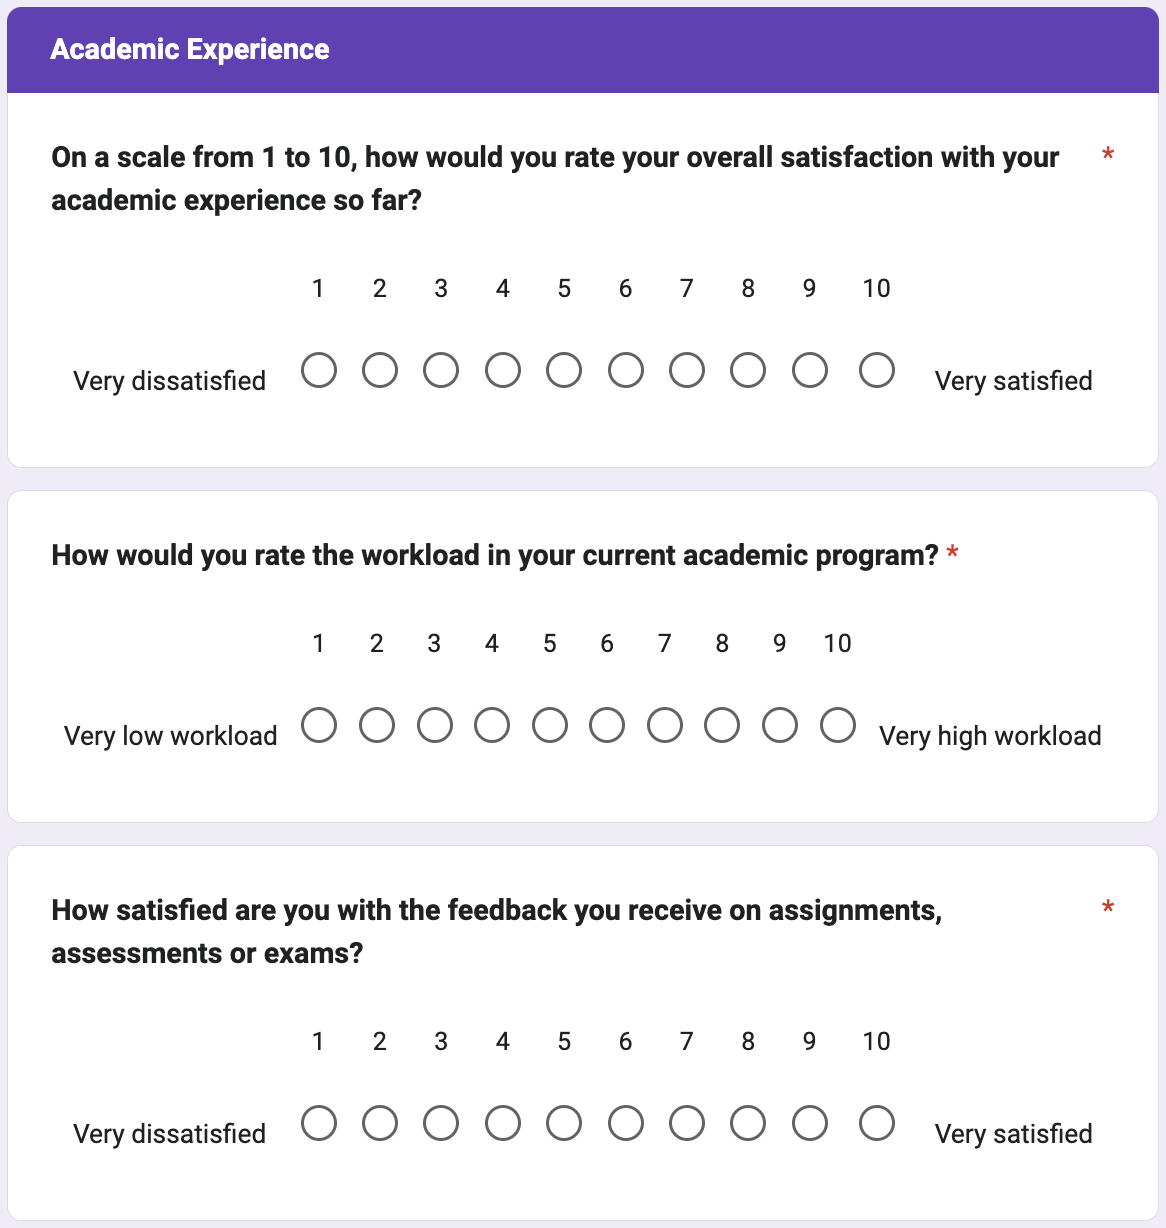
\includegraphics[width=0.49\linewidth]{figures/images/3.png}\label{fig:q3-1}}
    \hfill
    \subfloat[Part 2]{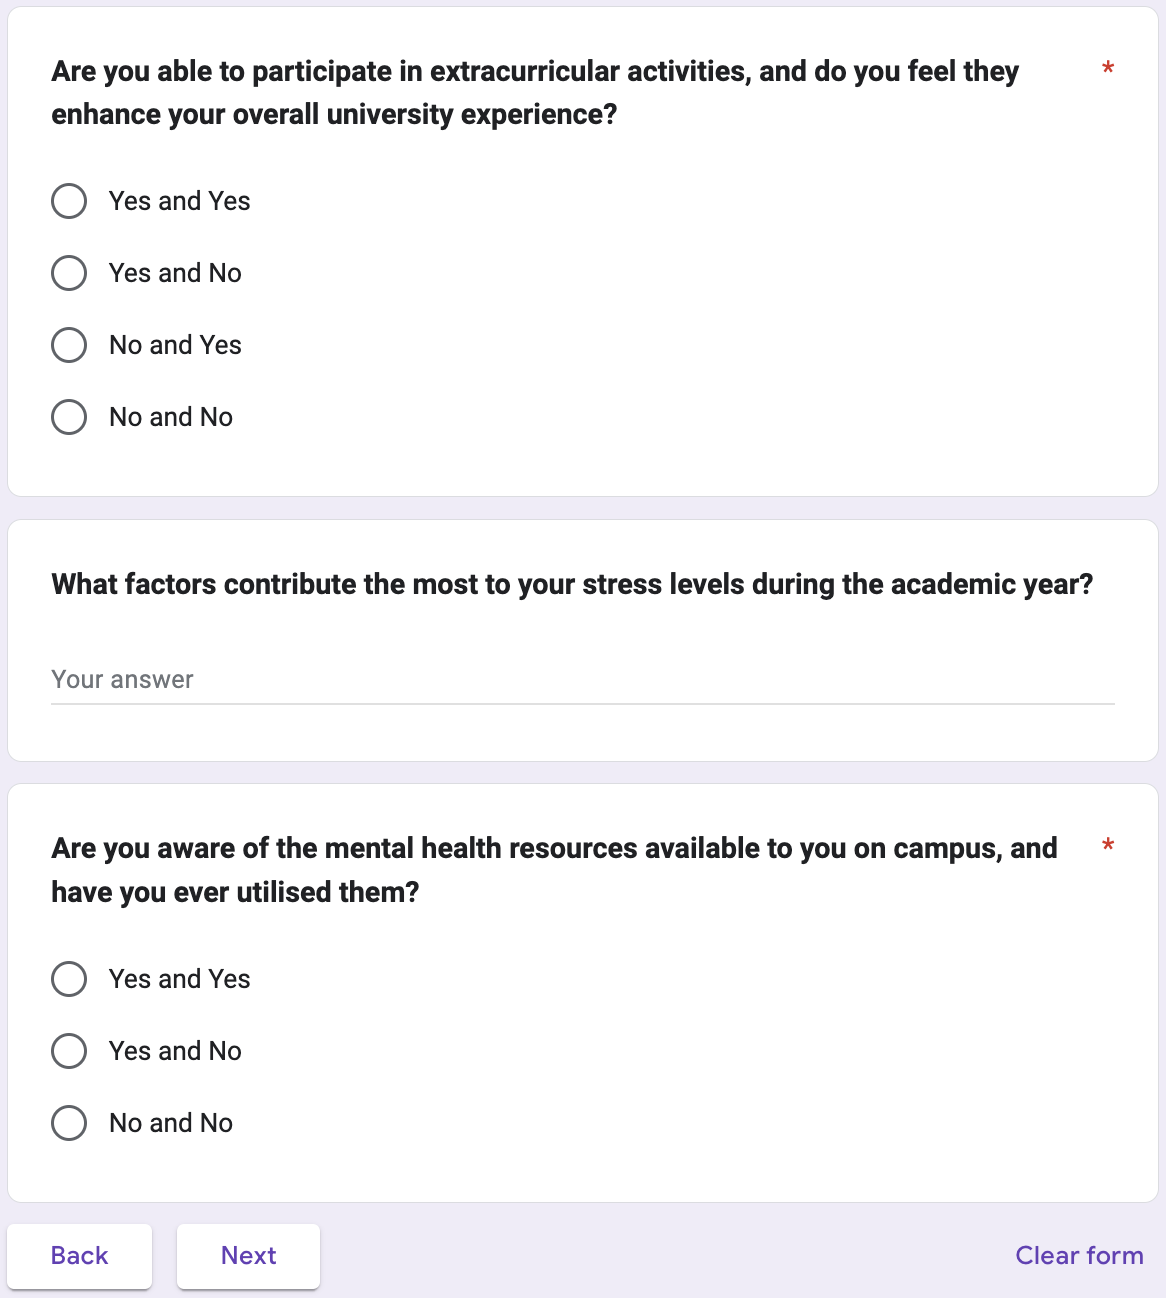
\includegraphics[width=0.46\linewidth]{figures/images/4.png}\label{fig:q3-2}}
    \caption{Third page of the survey}
    \label{fig:q3}
\end{figure}
\\The fourth page [\ref{fig:q4}] of the survey focuses on communication dynamics between students and professors. This section aims to uncover insights into the current state of communication between students and professors, allowing for a more detailed understanding of the communication challenges that may impact students' well-being.
\begin{figure}[h!]
    \centering
    \subfloat[Part 1]{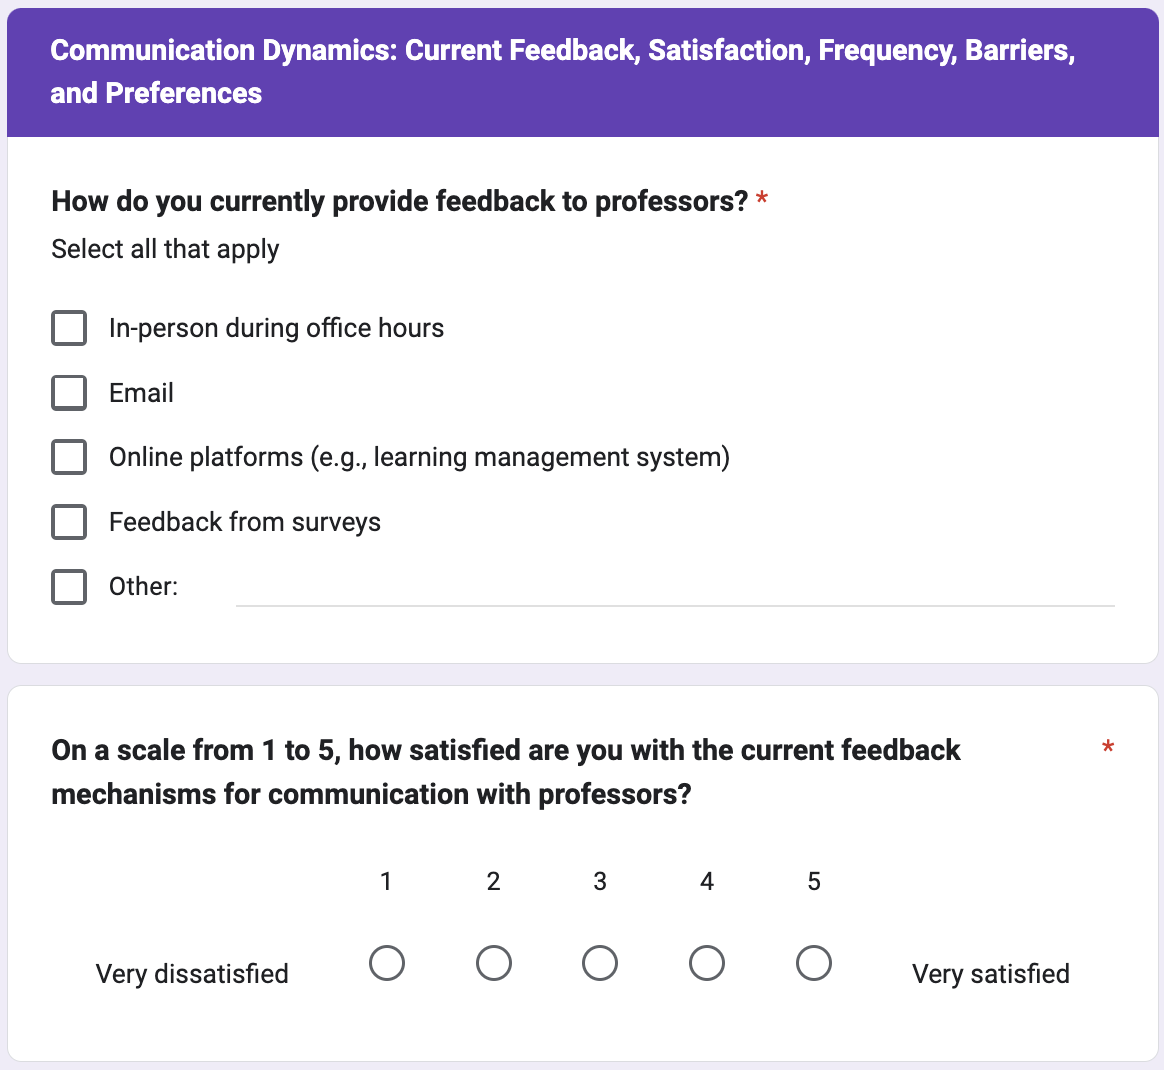
\includegraphics[width=0.48\linewidth]{figures/images/5.png}\label{fig:q4-1}}
    \hfill
    \subfloat[Part 2]{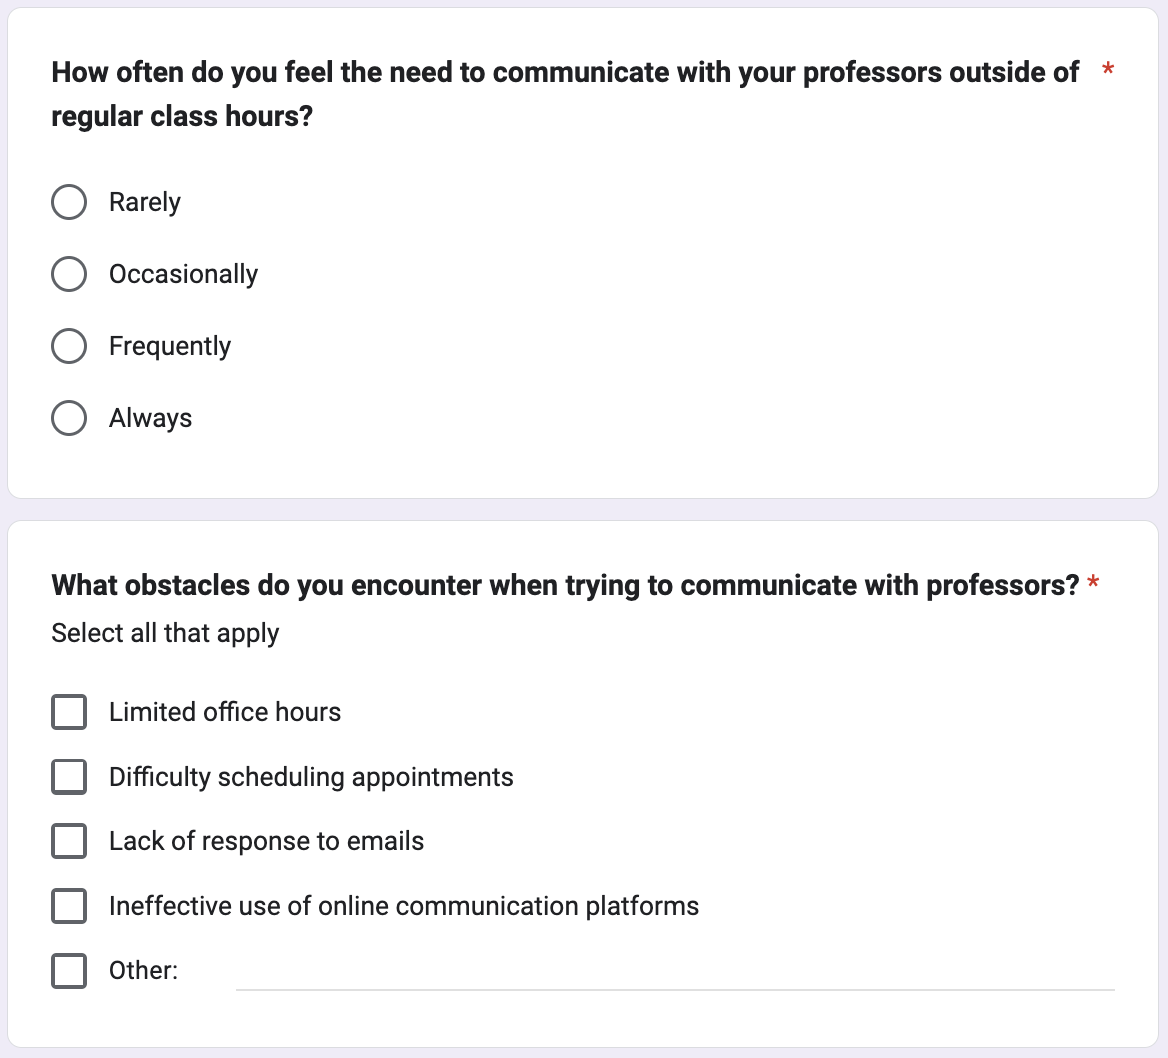
\includegraphics[width=0.49\linewidth]{figures/images/6.png}\label{fig:q4-2}}
    % Leave space between 1,2 and 3 for subfloat labels
    \vspace{0.5cm}
    \subfloat[Part 3]{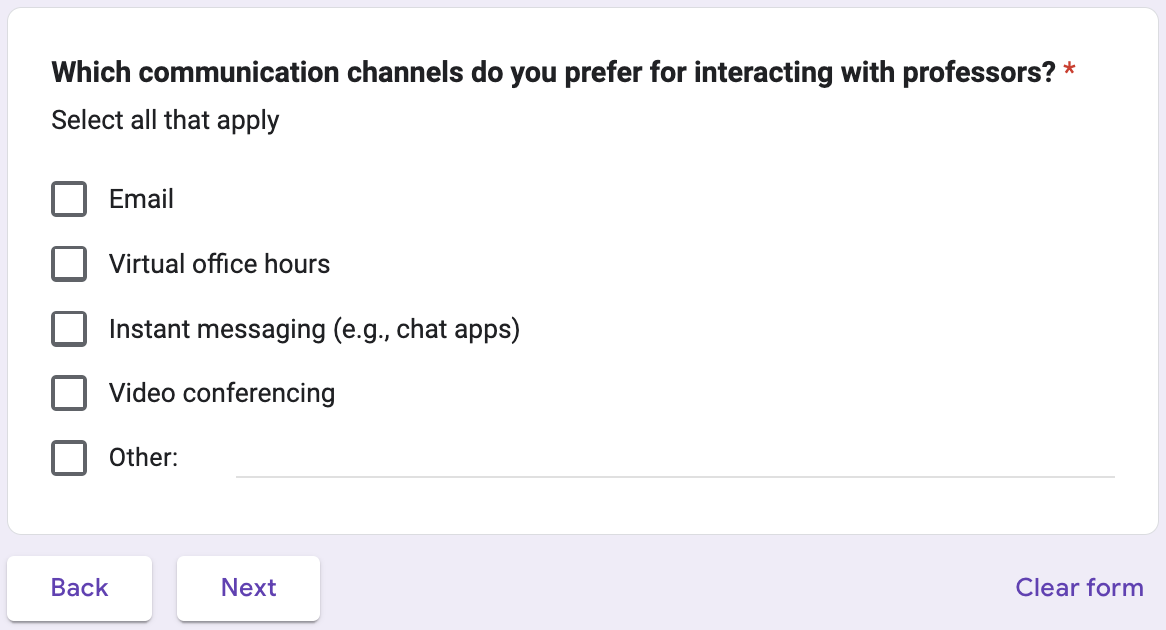
\includegraphics[width=0.60\linewidth]{figures/images/7.png}\label{fig:q4-3}}
    \caption{Fourth page of the survey}
    \label{fig:q4}
\end{figure} \\ \\ \\
The fifth page [\ref{fig:q5}] of the survey provides a valuable opportunity for participants to share their insights and contribute to the identification of actionable strategies for creating a more enriching and supportive academic environment.\vspace{5mm} \\
The sixth and final page [\ref{fig:q6}] of the survey gives participants the opportunity to share any additional thoughts or concerns they may have.
\begin{figure}[t!]
    \centering
    \subfloat[Fifth]{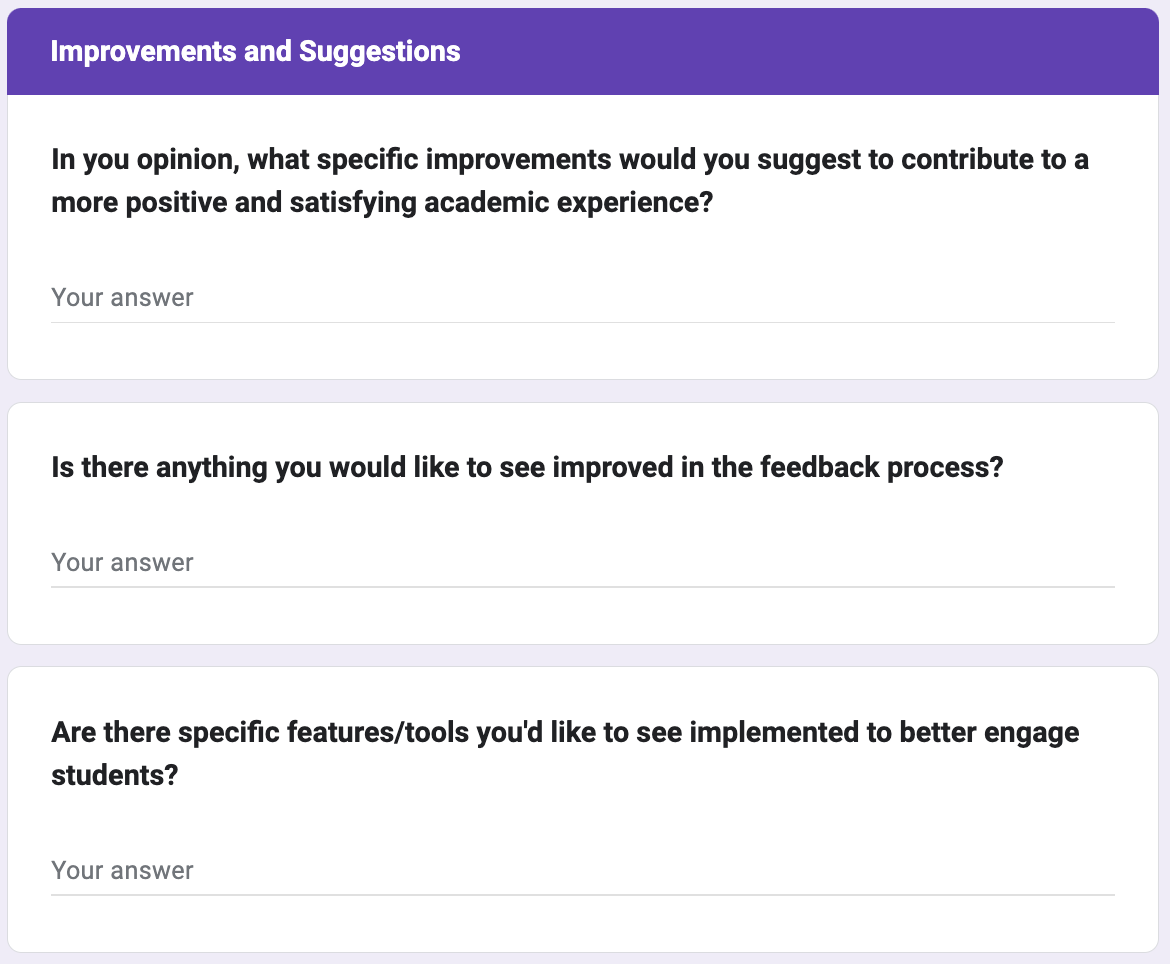
\includegraphics[width=0.46\linewidth]{figures/images/8.png}\label{fig:q5}}
    \hfill
    \subfloat[Sixth]{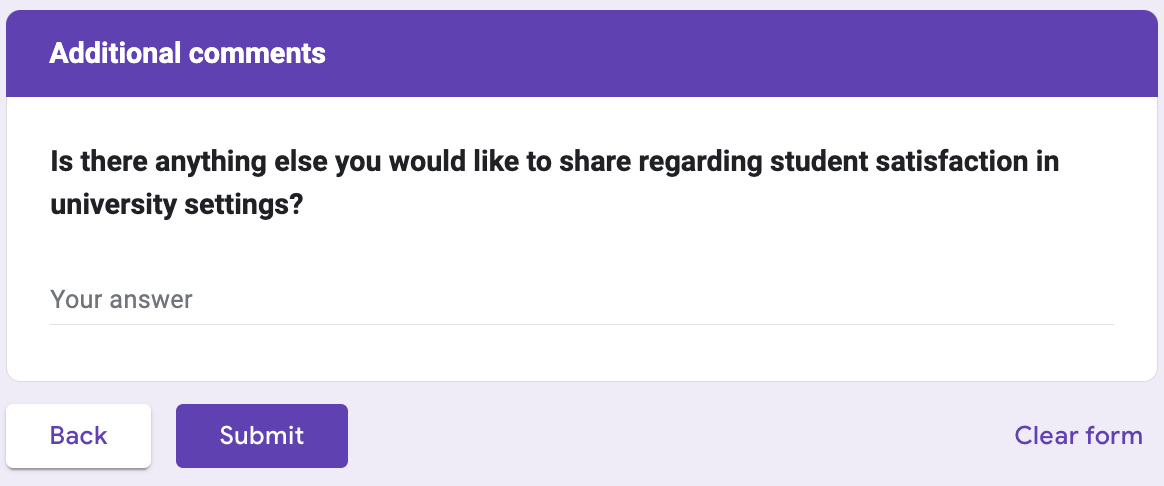
\includegraphics[width=0.50\linewidth]{figures/images/9.png}\label{fig:q6}}
    \caption{Fifth and sixth page of the survey}
\end{figure}

\chapterfont{\LARGE \centering}
\chaptertitlefont{\Large \centering}
\chapter{Scenarios - Model of future solution - Paper Mockups}


\chapterfont{\LARGE \centering}
\chaptertitlefont{\Large \centering}
\chapter{Creation and Evaluation of  Lo-Fi prototype}


\chapterfont{\LARGE \centering}
\chaptertitlefont{\Large \centering}
\chapter{Creation and Evaluation of  Hi-Fi prototype - Documentation for Developers - Presentation}

\printbibliography
\end{document}